
\documentclass[a4paper,10pt]{article}
   
\usepackage[T1]{fontenc}
\usepackage[utf8]{inputenc}
\usepackage{textcomp}
\usepackage[T1]{fontenc}
\usepackage{graphicx}
\usepackage{xcolor, colortbl}
\usepackage{caption}
\usepackage{listings}
\usepackage{wrapfig} 
\usepackage{tabu} % For coloring single row of table
\usepackage{scrextend}
\usepackage{hyperref}

\PassOptionsToPackage{hyphens}{url}\usepackage{hyperref}

\renewcommand\familydefault{\sfdefault} 
\usepackage{tgheros}


\usepackage{amsmath,amssymb,amsthm,textcomp}
\usepackage{enumerate}
\usepackage{multicol}
\usepackage{tikz}

\usepackage{geometry}
\usepackage{trace}
\usepackage{tcolorbox}
\usepackage{tabularx}
\usepackage{accsupp}% http://ctan.org/pkg/accsupp
\usepackage{enumitem}

%% For using numbers at every level of enumerated list
\newlist{legal}{enumerate}{10}
\setlist[legal]{label*=\arabic*.}

\tcbuselibrary{listings,skins} % For lstlisting

\geometry{total={210mm,297mm},
left=25mm,right=25mm,%
bindingoffset=0mm, top=20mm,bottom=20mm}


% For coloring single row in table
\def\zapcolorreset{\let\reset@color\relax\ignorespaces}
\def\colorrows#1{\noalign{\aftergroup\zapcolorreset#1}\ignorespaces}

\newcommand{\linia}{\rule{\linewidth}{0.5pt}}
\newcommand{\ano}{\text{3}}

% custom theorems if needed
\newtheoremstyle{mytheor}
    {1ex}{1ex}{\normalfont}{0pt}{\scshape}{.}{1ex}
    {{\thmname{#1 }}{\thmnumber{#2}}{\thmnote{ (#3)}}}

\theoremstyle{mytheor}
\newtheorem{defi}{Definition}

%%% Declare title %%%%%%%%%%%%%%%%%%%%%%%%%%%%%%%%%%%%%%%%%%%%%%%%
\newcommand{\antitle}{\text{Basics of Xilinx Vivado}}
% my own titles
\makeatletter
\renewcommand{\maketitle}{
\begin{center}
  \vspace{2ex} {\textsc{{{\large}Supplementary Material}\vspace{0.1cm}
      \break \huge \antitle}} \vspace{1ex}
  \\
%%%%%%%%%%%%%%%%%%%%%%%%%%%%%%%%%%%%%%%%%%%%%%%%%%%%%%%%%%%%%%%%%%

Department of Electronics and Communication Engineering \\
Indian Institute of Technology, Roorkee
\linia\\
ECN 104 \hfill Digital Logic Design
\vspace{4ex}
\end{center}
}
\makeatother
%%%

% custom footers and headers
\usepackage{fancyhdr}
\pagestyle{fancy}
\lhead{}
\chead{}
\rhead{}
\lfoot{Assignment \ano\ - \antitle}
\cfoot{}
\rfoot{Page \thepage}
\renewcommand{\headrulewidth}{0pt}
\renewcommand{\footrulewidth}{0pt}
%

\definecolor{vgreen}{RGB}{104,180,104}
\definecolor{vblue}{RGB}{49,49,255}
\definecolor{vorange}{RGB}{255,143,102}

\makeatletter
\newcommand*\@lbracket{[}
\newcommand*\@rbracket{]}
\newcommand*\@colon{:}
\newcommand*\colorIndex{%
    \edef\@temp{\the\lst@token}%
    \ifx\@temp\@lbracket \color{black}%
    \else\ifx\@temp\@rbracket \color{black}%
    \else\ifx\@temp\@colon \color{black}%
    \else \color{vorange}%
    \fi\fi\fi
}
\makeatother

\definecolor{codebg}{RGB}{250,250,240} 
\definecolor{greatblue}{RGB}{91,155,215} 

% Set up caption and labels for lstlistings
\DeclareCaptionFont{white}{\color{white}}
\DeclareCaptionFormat{listing}{\colorbox{greatblue}{\parbox{\textwidth}{\hspace{1cm}#1#2#3}}}
\captionsetup[lstlisting]{format=listing,labelfont=white,textfont=white}

\renewcommand{\thelstnumber}{% Line number printing mechanism
  \protect\BeginAccSupp{ActualText={}}\arabic{lstnumber}\protect\EndAccSupp{}%
}

\def\backtick{\char18} 
\lstdefinestyle{verilog-style}
{
    %columns=fullflexible, 
    language=Verilog,
    basicstyle=\small\ttfamily,
    keywordstyle=\color{vblue},
    identifierstyle=\color{black},
    commentstyle=\color{vgreen},
    numbers=left, 
    numberstyle=\color{gray},  
    numbersep=10pt,
    moredelim=*[s][\colorIndex]{[}{]},
    literate=*{:}{:}1, 
%    backgroundcolor=\color{codebg},
%    framexrightmargin=0.09cm, 
    framexleftmargin=-0.09cm,
    frame=trbl,
    upquote=true, 
    framerule=0pt,
    keepspaces=true
}

\lstdefinestyle{verilog-inline-style}
{
    language=Verilog,
    basicstyle=\small\ttfamily,
    keywordstyle=\color{vblue},
    identifierstyle=\color{black},
    commentstyle=\color{vgreen},
    moredelim=*[s][\colorIndex]{[}{]},
    literate=*{:}{:}1, 
    upquote=true, 
    framerule=0pt,
    keepspaces=true
}

\newcommand{
  \insertverilog}[3]{
  \lstinputlisting[label=#2, caption=#3, style={verilog-style}]{#1}
}


% Command for problem
\newcounter{problemNumber}
\setcounter{problemNumber}{1}
\newcommand {
  \insertProblem}[1]{
  \vspace{0.5cm}
  \hrule
  \vspace{0.3cm}

  {\color{greatblue}\textbf{\large{Problem \theproblemNumber}}}
  \vspace{2pt}\\#1

  \addtocounter{problemNumber}{1}
  \vspace{0.2cm}
  \hrule  
  \vspace{0.5cm}
}


%%%----------%%%----------%%%----------%%%----------%%%
% Command for creating a resource box
\newcommand{\resourcebox}[2]{
  \fbox{%
    \parbox{0.5\textwidth}{%
      \text{#1}
    }%
  } 
}


%%%----------%%%----------%%%----------%%%----------%%%
% Command for creating circled numerals
\usepackage{tikz}
\usepackage{xcolor}
\newcommand*\circled[1]{\tikz[baseline=(char.base)]{
            \node[shape=circle,fill,inner sep=2pt] (char) {\textcolor{white}{#1}};}}

%%%----------%%%----------%%%----------%%%----------%%%
% Setups hyper
\hypersetup{
  colorlinks=true,
  allcolors=blue
}

%%%----------%%%----------%%%----------%%%----------%%%

\makeatletter
\def\lst@outputspace{{\ifx\lst@bkgcolor\empty\color{white}\else\lst@bkgcolor\fi\lst@visiblespace}}
\makeatother

%%%----------%%%----------%%%----------%%%----------%%%
\begin{document}

\maketitle

\section*{Creating a New Project}
To create a new project follow the instructions from this YouTube
tutorial:

\begin{enumerate} \item[] \url{https://youtu.be/wqm2dgQsj_A} \end{enumerate}

\section*{Vivado GUI guide}
This section explains the basic of Xilinx Vivado GUI, this section
provides only the basic explanation to get you started and is not an
exhaustive list of all the feature. Please refer to the Vivado
User Guide for more information.

\begin{figure}[!h] \centering  
  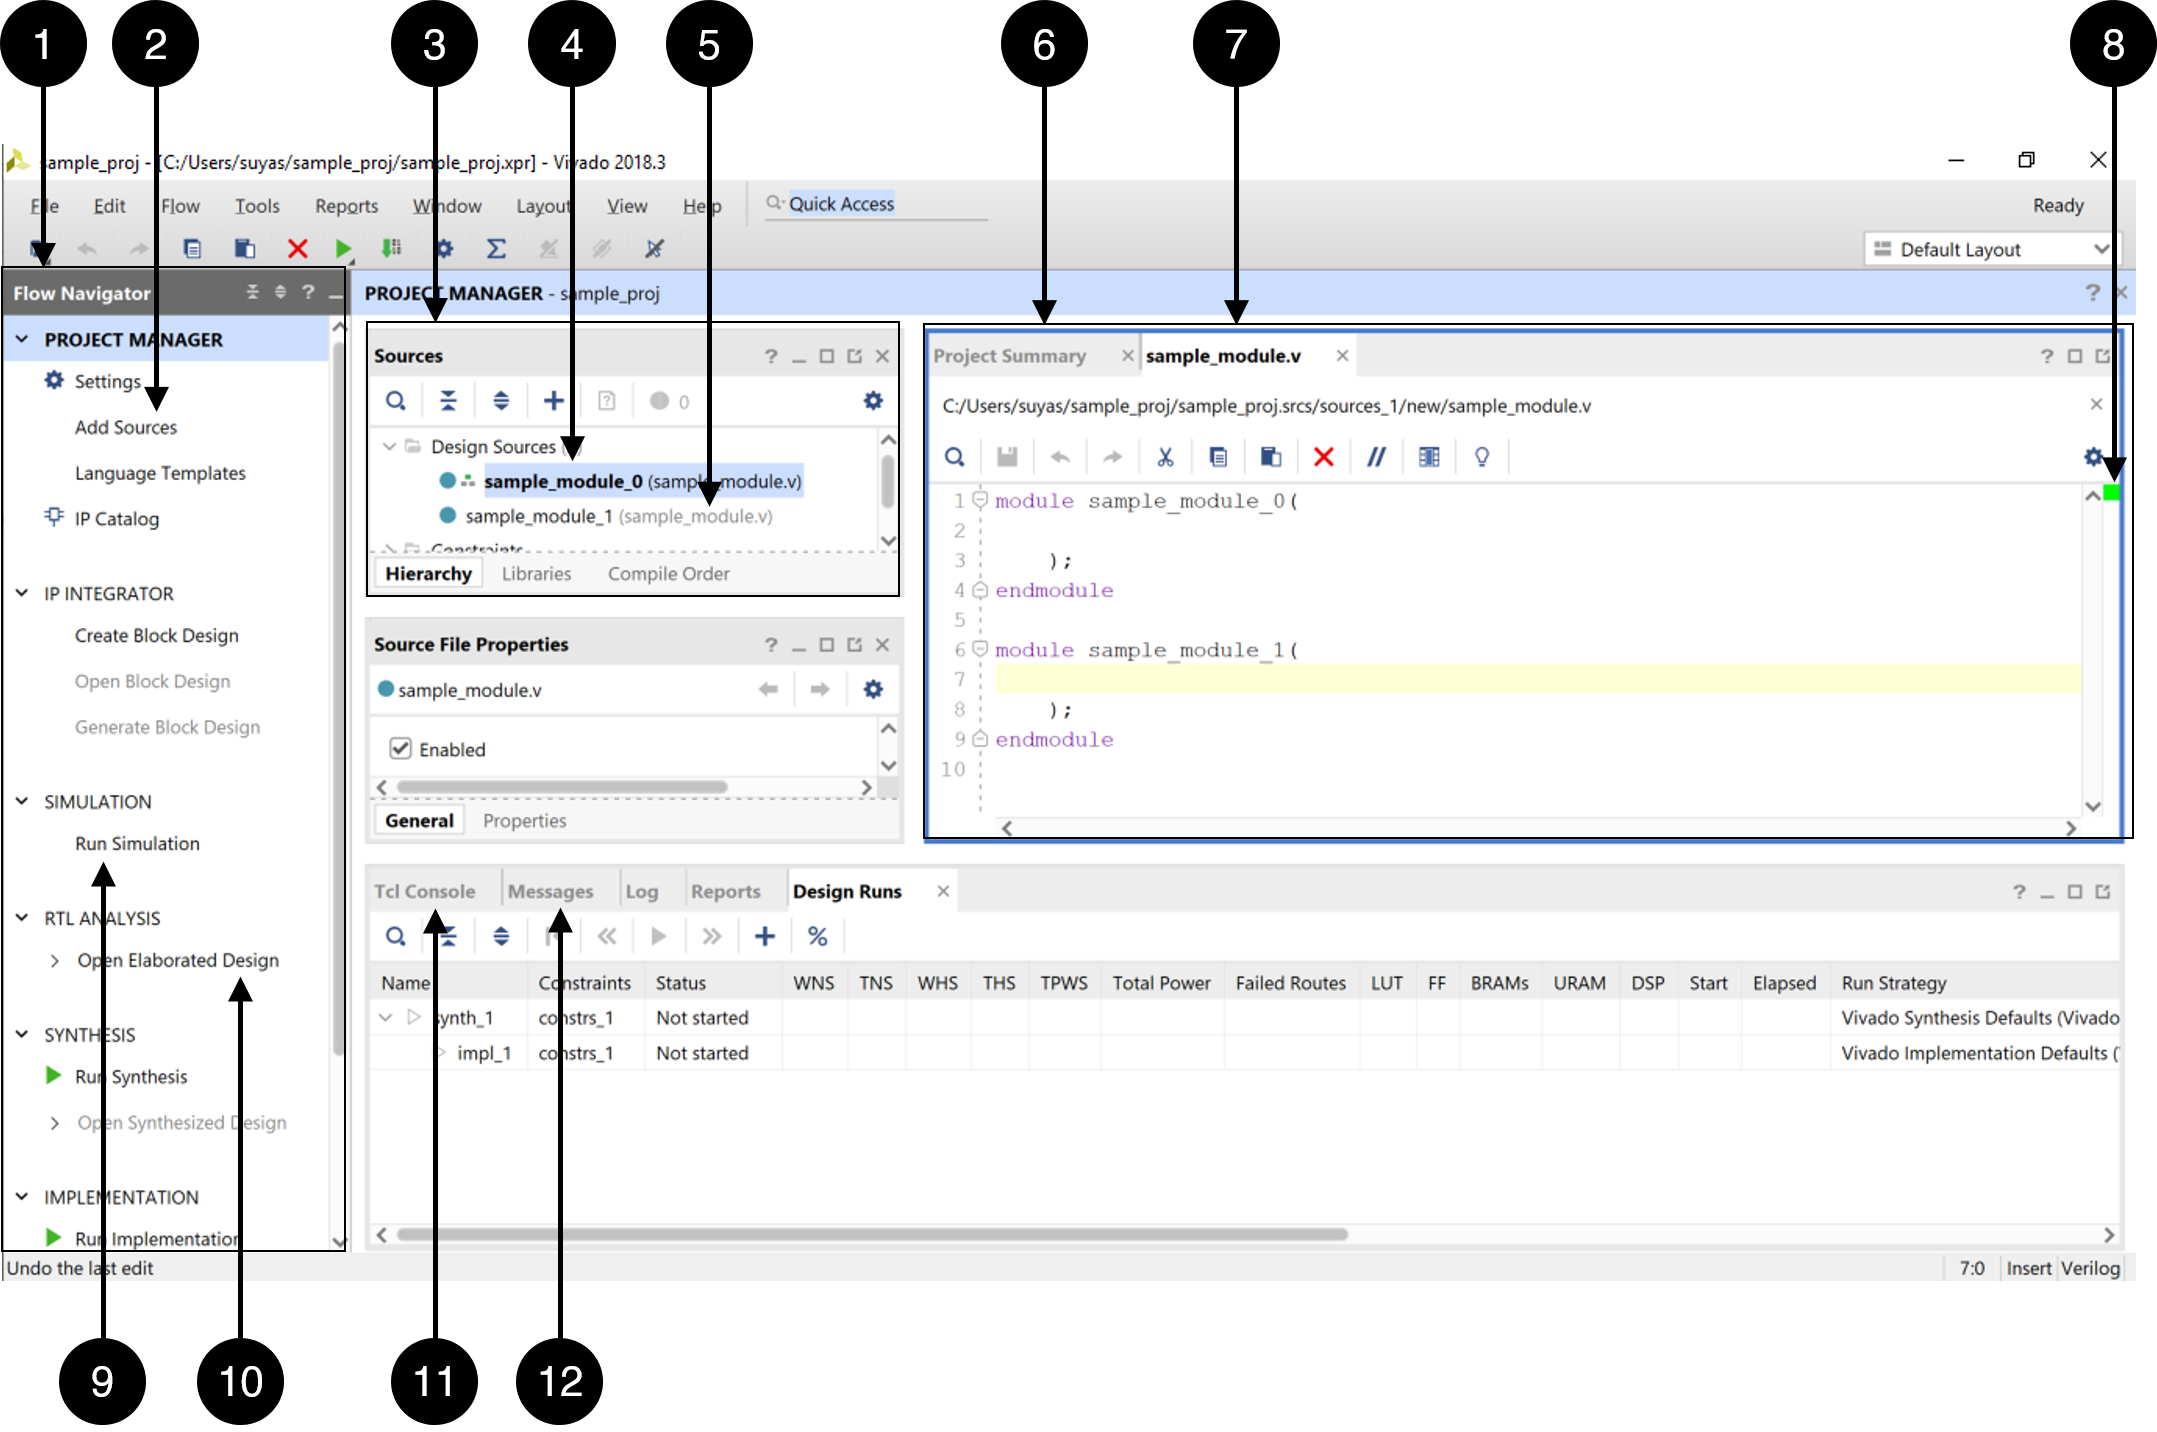
\includegraphics[width=\linewidth]{./img/vivado_gui.png}
  \caption{Overview of Xilinx Vivado GUI.} 
  \label{fig:vivado-gui}
\end{figure}

Fig. \ref{fig:vivado-gui} shows the overview of Xilinx Vivado 2018.3
GUI, the important sections of the GUI are explained below:
\begin{itemize}
\item[] \circled{1} \textbf{Flow Navigator} Pane contains the options
  for different operations during a common design flow this includes
  option to include new source files (\circled{2}), run simulation
  (\circled{9}) or to open elaborated design (\circled{10}).
\item[] \circled{2} \textbf{Add Sources} option allows adding creating
  new source files/adding existing files to the project.
\item[] \circled{3} \textbf{Sources} pane lists all the modules in the
  project along with the file they belongs to in a hierarchical
  fashion.
\item[] \circled{4} \textbf{Current Top Module}'s name is listed in
  bold face. Both \textit{Design Sources} and \textit{Simulation
    Sources} have their corresponding top level modules. Top level
  module in \textit{Simulation Sources} is used for simulation and top
  level modules from \textit{Design Sources} is used for generating
  elaborated design.
\item[] \circled{5} \textbf{Other modules} which are not top level
  module are shown in normal face (unlike \circled{4}).
\item[] \circled{6} \textbf{Workspace} in Vivado contains all the
  schematic, text editors and simulation windows unless undocked.
\item[] \circled{7} \textbf{Text editor} currently selected is
  highlighted with the file's name in bold face. If the file is
  unsaved an asterisk(\textbf{*}) will appear next to the name.
\item[] \circled{8} \textbf{Green square} next to the scroll bar
  indicates that the code is free from common syntax errors. This
  square turns red if the source code has syntax errors. Please note
  that this feature is just for indication of possible syntax errors,
  even though if the square is green your code might be logically
  incorrect or might be syntactically incorrect.
\item[] \circled{9} \textbf{Run Simulation} allows you to run
  simulation using the currently selected top level module in
  simulation sources. A new window is opened in the Workspace
  (\circled{6}) to view the waveforms.
\item[] \circled{10} \textbf{Open Elaborated Design} generates the
  schematic representation of your design.
\item[] \circled{11} \textbf{Tcl Console} contains log of all the
  errors and warnings generated during past operations (you might have
  to scroll through several lines before finding the relevant
  warning/error).
\item[] {\small\circled{12}} Vivado reads the Tcl console output to list
  common errors and warnings as a user friendly format in
  \textbf{Message} Pane. Please note that you might still have to
  access the \textit{Tcl Console} pane for finding information on
  errors.
\end{itemize}

\section*{Adding an Existing Testbench To Your Project}
To add an existing testbench to your code follow the instructions from
this YouTube tutorial:

\begin{enumerate} \item[] \url{https://youtu.be/wqm2dgQsj_A} (Using
  existing testbench with Vivado) \end{enumerate}

\section*{Document History}
\begin{enumerate}
\item \textbf{Mon Feb  4 10:25:06 IST 2019}: First edition

\end{enumerate}
\end{document}
